\section{Methodology}\label{sec:method}

Here we are going to introduce methods we used to select variables. 

As described in \eqref{eq:model}, we are facing a linear regression model in high dimensional space with multiple response variables. 
This makes it more difficult for us to deal with problems. 

Next, we will introduce three methods to solve the model. 
They were verified as a good method to deal with univariate high-dimensional linear regression, grouped variables, and factorization problem. 

\subsection{Unit-Response Regression}

Denote $Y_j$ as the $j$-th colume of $Y$, which represents the expression level of $j$-th gene. 

It is intuitive for us to divide and conquer it by regressing each $Y_j$ with $X$ and and we will get $q$ linear models. 

We can use classical LASSO \citep{tibshirani1996regression} to get the estimated coefficient vector $\hat{\beta}_{\cdot j} \in \mathbb{R}^{p}$. 
Then combine $q$ coefficient vectors $\hat{\beta}_{\cdot j}$ into a matrix $\widehat{B}\in\mathbb{R}^{p\times q}$ by column. 

\begin{figure}[ht]
    \centering
    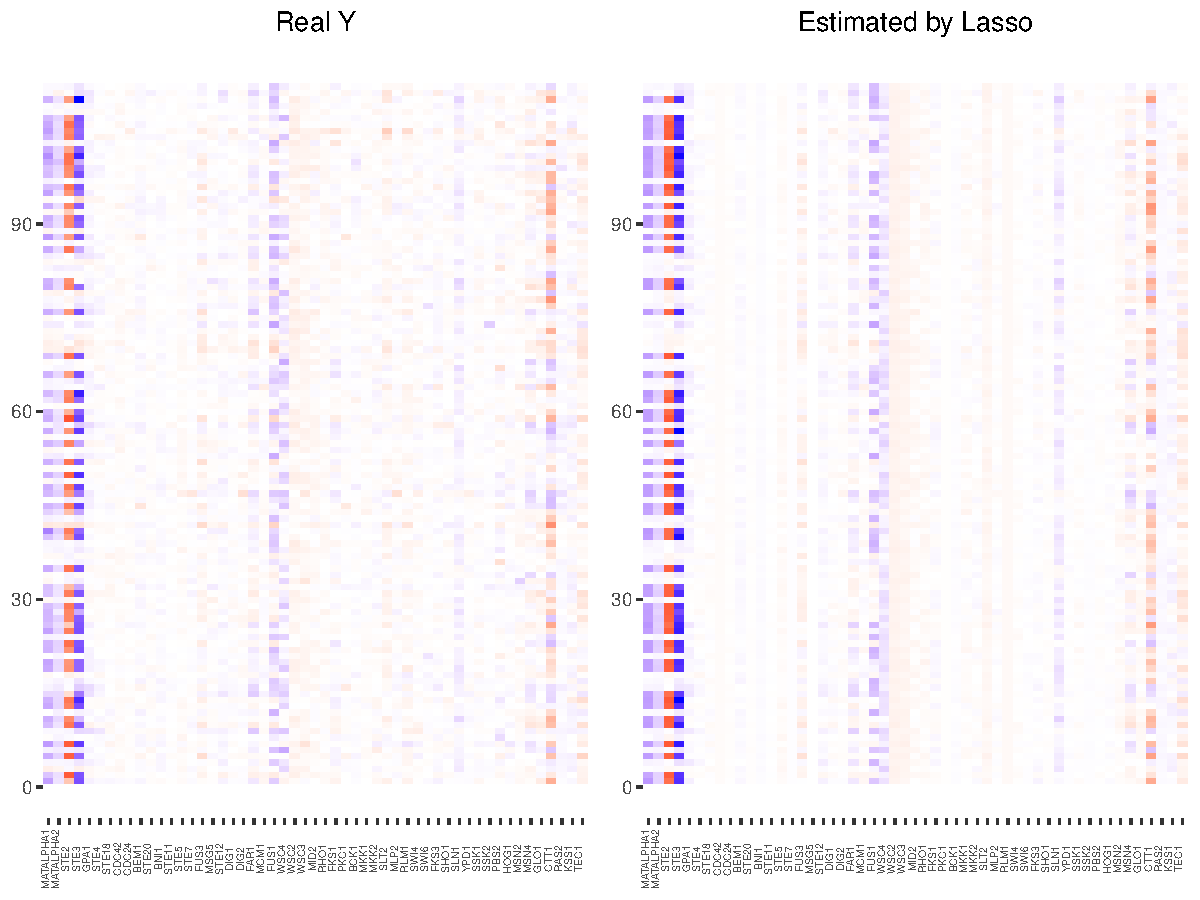
\includegraphics[width=0.7\textwidth]{./figs/heatmap_lasso.pdf}
    \caption{Heatmaps of real $Y$ and $\hat{Y}$ by LASSO}
    \label{fig:heatmaplasso}
\end{figure}

We plot heatmap of predicted $Y$ and the real one in Figure~\ref{fig:heatmaplasso} because it is simpler and more intuitive than displaying numbers. 
We can learn from the diagram that the two colors are almost the same, indicating that the estimation results by LASSO are acceptable. 


However, as is known, LASSO is a kind of shinkage estiamtion method with $L_1$ penalty, which not only shrinks the size of the coefficients, but also set some of them to zero. 
So a sparse $\hat{\beta}_{\cdot j}$ is expected for each $j\in\{ 1,2,\dots,q \}$. 
We rewrite the optimazation function as following
\begin{equation}
    \widehat{B}=\underset{B}{\arg \min }\left\{\frac{1}{2n}\|Y-X B\|_{F}^{2} + \sum_{i=1}^q \lambda_i \|B_{\cdot i}\|_{1} \right\}
\end{equation}
where $\|\cdot\|_{F}$ is the Frobenius norm and $\sum_{i=1}^q \lambda_i \|B_{\cdot i}\|_{1}$ can be regraded as a $(1,1)$ norm of matrix $B$. 

Actually, we got $602$ nonzero rows in $\widehat{B}$ which also has full column rank. 



\subsection{Grouped-Response Regression}

Group sparse linear regression for multitask learning \citep{dai2016knockoff}
\begin{equation}
    \widehat{B}=\underset{B}{\arg \min }\left\{\frac{1}{2n}\|Y-X B\|_{F}^{2} + \lambda \|B\|_{(2,1)}\right\}
\end{equation}
where the $(2,1)$ norm in the penalty is given by
$\|B\|_{(2,1)} = \sum_i \sqrt{\sum_j B_{ij}^2}$.

\begin{figure}[ht]
    \centering
    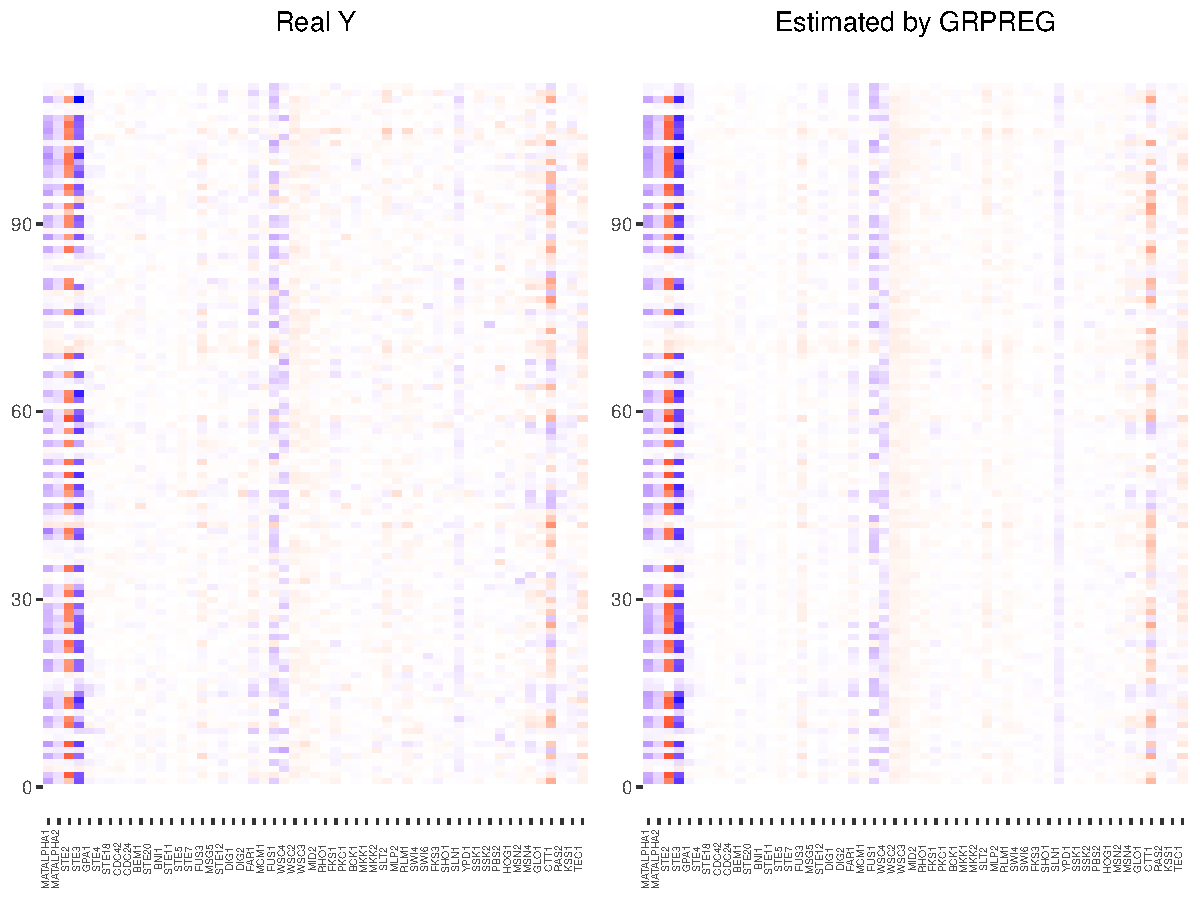
\includegraphics[width=0.7\textwidth]{./figs/heatmap_grpreg.pdf}
    \caption{Heatmaps. $\widehat{B}$ has full column rank and 201 non-zero rows.}
    \label{fig:heatmapgroup}
\end{figure}

As shown in the Figure~\ref{fig:heatmapgroup}, although it totally uses fewer predictors variables than LASSO, but it also restores $Y$ well. 

Intuitively, $(2,1)$ norm penalty can be understood as a $L_1$ penalty imposed on sum of squares of the rows of $B$. 
If we choose a large $\lambda$, $\widehat{B}$ will contain many zero rows, however the nonzero rows will themselves be dense (not entrywise sparsity). 
This is because $(2,1)$ norm penalty promotes rowwise sparsity of $\widehat{B}$. 

Biologically, the result shows that among all $p$ markers, a total of $201$ markers are related to $53$ genes. 
And each marker selected has some effect on each gene in our data.



\subsection{Multi-Response Regression}

Previous biological research has revealed some facts which could be the guidelines for us to choose suitable method of data analysis.

Extensive genetic and biochemical analysis has revealed that there are a few functionally distinct signaling pathways of genes \citep{gustin1998map, brem2005landscape}, suggesting that the association structure between the eQTLs and the genes is of low rank. 
Each signaling pathway involves only a subset of genes, which are regulated by only a few genetic variants, suggesting that each association between the eQTLs and the genes is sparse in both the input and the output (or in both the responses and the predictors), and the pattern of sparsity should be pathway specific. 
Moreover, it is known that the yeast MAPK pathways regulate and interact with each other \citep{gustin1998map}. 

The complex genetic structures described above clearly indecate that the association structure between the eQTLs and the gene is of low rank and sparsity. It call for a joint statistical analysis that can reveal multiple distinct associations between subsets of genes and subsets of genetic variants. 

SOFAR \citep{uematsu2019sofar} uses the SVD decomposition $B= UDV^T$ and then impose penalties into $U$, $D$ and $V$ respectively. 
\begin{equation} % \footnotesize
    \begin{split}
        \left( \widehat{D}, \widehat{U}, \widehat{V} \right) 
        = & \underset{D, U, V}{\arg \min }\left\{\frac{1}{2n} \left\|X- UDV^{T}\right\|_{F}^{2} + \lambda_{d}\|D\|_{1}+\lambda_{a} \rho_{a}(U D)+\lambda_{b} \rho_{b}(VD)\right\} \\ 
        & \quad\quad\quad \text { subject to } U^{T} U=\mathbf{I}_{m}, \quad V^{T} V=\mathbf{I}_{m} 
    \end{split}
\end{equation}

Rank reduction is achieved mainly through the first term and variable selection is achieved through the last two terms. 
$\rho_a(\cdot)$ and $\rho_b(\cdot)$ can be equal or distinct, depending on our questions and goals. 
$\rho$ can be entrywise $L_1$ norm or rowwise $(2, 1)$ norm or others.

Figure~\ref{fig:heatmapsofar} shows the results from SOFAR with turning parameters $\lambda_{d}$, $\lambda_{a}$ and $\lambda_{b}$ choosen by cross validation. 
SOFAR returned rowwise sparse singular matrix $U$ and $V$ and a low rank diagram matrix $D$. 
It finds only $228$ significant markers by selecting non-zero rows in the estimation of $U$, $25$ genes by selecting non-zero rows in the estimation of $V$ and $3$ latent patterns within the data. 

\begin{figure}[ht]
    \centering
    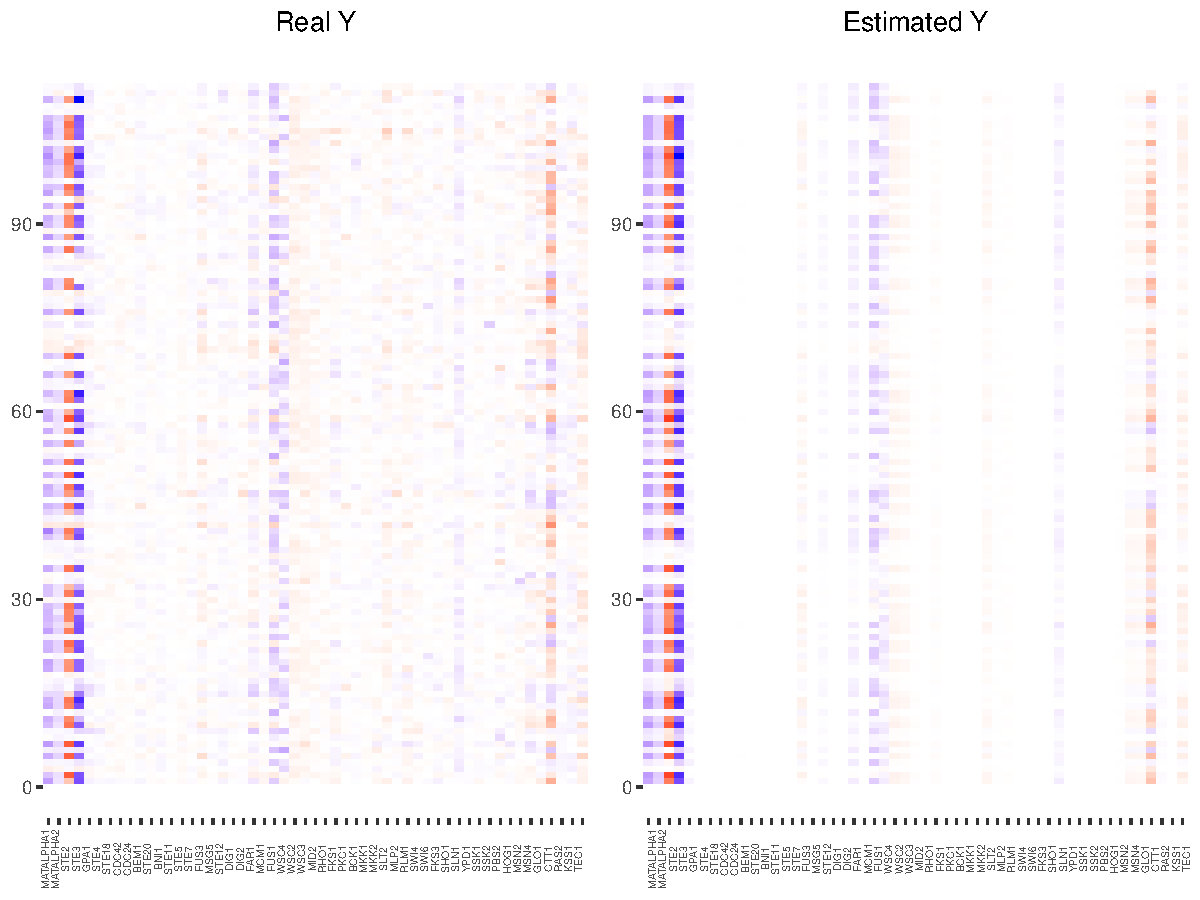
\includegraphics[width=0.7\textwidth]{./figs/heatmap1.pdf}
    \caption{Heatmaps of real $Y$ and $\hat{Y}$ by SOFAR}
    \label{fig:heatmapsofar}
\end{figure}

Specifically, the rank of coefficient matrix is $3$, as shown in the Figure~\ref{fig:scatter}, indicating that there are only three latent variables ($XU$). 
Figure~\ref{fig:scatter} shows the specific linear relationship between $XU$ and response variables $YV$ in different patterns, and the fitting is pretty good. 
And here we also get the sparsity of $U$ and $V$. 

\begin{figure}[ht]
    \centering
    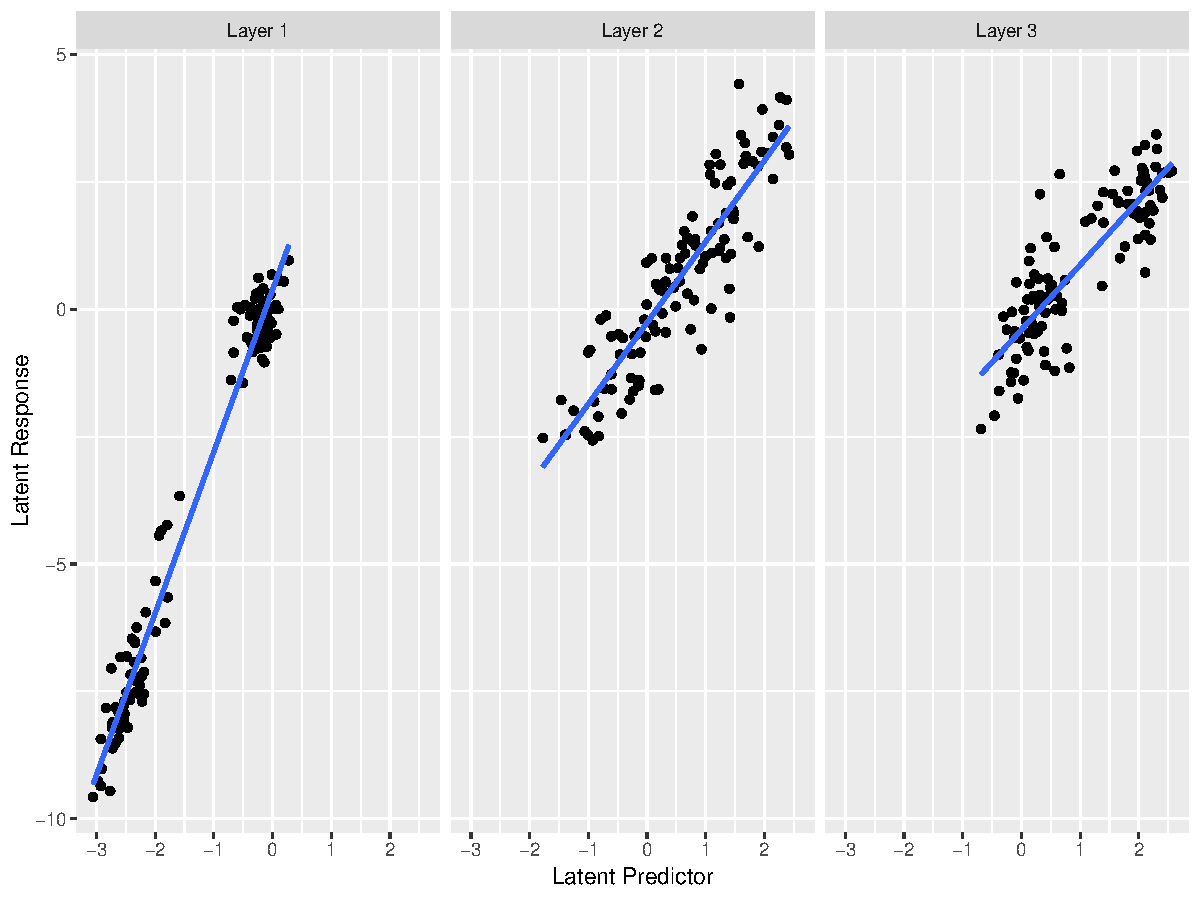
\includegraphics[width=0.65\textwidth]{./figs/latent1.pdf}
    \caption{Scatter plots of the latent responses versus the latent predictors in three SVD layers for the yeast data estimated by the SOFAR method}
    \label{fig:scatter}
\end{figure}



\begin{figure}[ht]
    \centering
    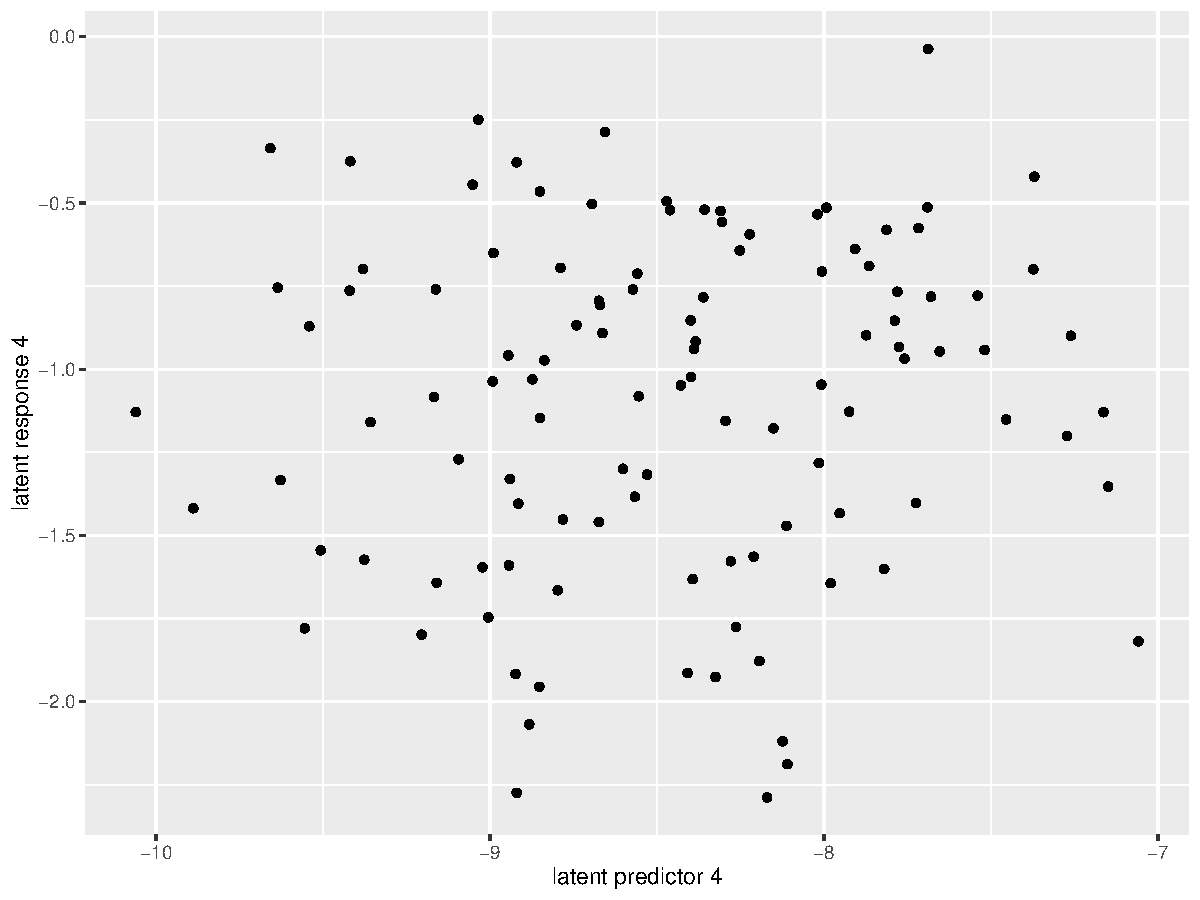
\includegraphics[width=0.65\textwidth]{./figs/latent4.pdf}
    \caption{Scatter plots of the $4$th latent responses versus the latent predictors for the yeast data estimated by the SOFAR method}
    \label{fig:4th-pattern}
\end{figure}

In order to check whether the SOFAR method completely finds the letent pattern within the data, we drew the fourth possible latent pattern in Figure~\ref{fig:4th-pattern}. 
As is shown, the latent response and the latent predictor are almost completely independent and there is no possible relationship.